\chapter{State of the Art\label{cha:chapter2}}

\section{Live Streaming\label{sec:live}}

\todo[inline]{reference dash and hls from Bachelor}
% TODO re-do this, more detailed
For more than 15 years HAS has been the defacto standard media streaming protocol. Media that is streamed this way is transcoded into a number of different tracks. For video these tracks usually represent different qualities, for example bitrate and resolution, audio can also have different qualities levels but also different languages. These tracks are then separated into small chunks, usually a few seconds of length.

Each stream has a manifest which acts as the primary entry point. It contains general metadata about the stream as well as the available track options, including the request URIs, bitrate, resolution, sampling rate, frame per second, language and more data about the tracks.

A typical process begins with the player requesting the manifest. The player then uses the information found in the manifest to decide on which tracks to use first. Then it requests media segments and plays them back. In the meantime a player runs adaptive bitrate (ABR) algorithms to decide whether or not to change the track. An ABR algorithm can take many different aspects into consideration, like current download rate, buffer size, available qualities, segment length, etc. 

\todo[inline]{initialization segment definition}

% TODO specific subsection for dash and hls is overkill, only real difference is MPD vs M3U8 Playlist (and dash.js vs hls.js I guess)

\subsection{DASH\label{sub:dash}}

going over the specifics of DASH

\subsection{HLS\label{sub:hls}}

going over the specifics of HLS

\subsection{Content Provenance\label{sec:conpro}}

\section{C2PA\label{c2pa}}

\todo[inline]{How to reference the C2PA spec for this entire section?}
quick history of C2PA then going over the important parts of the spec in detail: Claim, Manifest, Content Types, etc.

\subsection{Manifest}

\subsubsection{Claim Signature}

\subsubsection{Claim}

\subsubsection{Assertions}

\subsection{BMFF Hashing}

The current C2PA specification version 2.1 describe version 3 of hashing BMFF content \footnote{BMFF-Based Hash V3 \url{https://c2pa.org/specifications/specifications/2.1/specs/C2PA_Specification.html\#_bmff_based_hash}}. However, since the implementation I used was version 2 at the time of forking, I will from here on refer to version 2 and describe its workings. Version 2 of BMFF hashing was specified in the C2PA specifications of the same version \footnote{BMFF.Based Hash V2 \url{https://c2pa.org/specifications/specifications/2.0/specs/C2PA_Specification.html\#_bmff_based_hash}}.

All information related to the hashing of BMFF content is written to the C2PA manifest as part of the Assertion with the label "\texttt{c2pa.hash.bmff.v2}".

% this is more complicated than I expected, don't sure if I'll want to describe this in detail, maybe towards the end if the thesis could use more text

> special case of hashing (include box location in hash)



\subsection{Merkle Tree\label{sec:merkle}}

A Merkle Tree can be used to create a signature of a large dataset by fragmenting it into smaller pieces. Then it is possible to validate one of these pieces as part of the whole dataset without needing to have access to the entire dataset. The C2PA specifications use a Merkle Tree for fragmented BMFF media.

A Merkle Tree is built from the bottom up. The first row of a Merkle Tree are the leaves. The leaves are the fragmented dataset, in this case the media segments, more specifically the leaves are the data hashes of the data. The next row are the parents of the previous row. If a parent node has both left and right children then the data hash of the parent node is the hash of the two children hashes concatenated, otherwise the children node hash is copied. This is repeated until the row with only a single node has been reached, this node is the root of the Merkle Tree \cite{merkle}.

Once the Merkle Tree is fully built only one of the layers has to be kept in memory, calling it reference tree layer from here on. Which layer is up to the application. The weight between number of hashes remembered and number of steps required for validation has to be considered for choosing the which layer to keep. Additionally, proof hashes are assigned to each leaf. These proofs are hashes that are part of the full Merkle Tree and they are the hashes are required to validate a leaf. They are the sibling nodes along the path from the leaf up to the reference tree layer.

A simple example of this can be seen in \Cref{fig:merkle_example}. For example the hash \texttt{H3} is the resulting hash of the concatenation of fragment hashes \texttt{F5} and \texttt{F6}, while the hash \texttt{H9} is the result from the hashes \texttt{H6} and \texttt{H7}. The fragment hash \texttt{F11} and hash \texttt{H8} are examples of the case where there is one child missing and that node is simply copied. In this example hash \texttt{H10} is the root of the Merkle Tree.

\begin{figure}
    \centering
    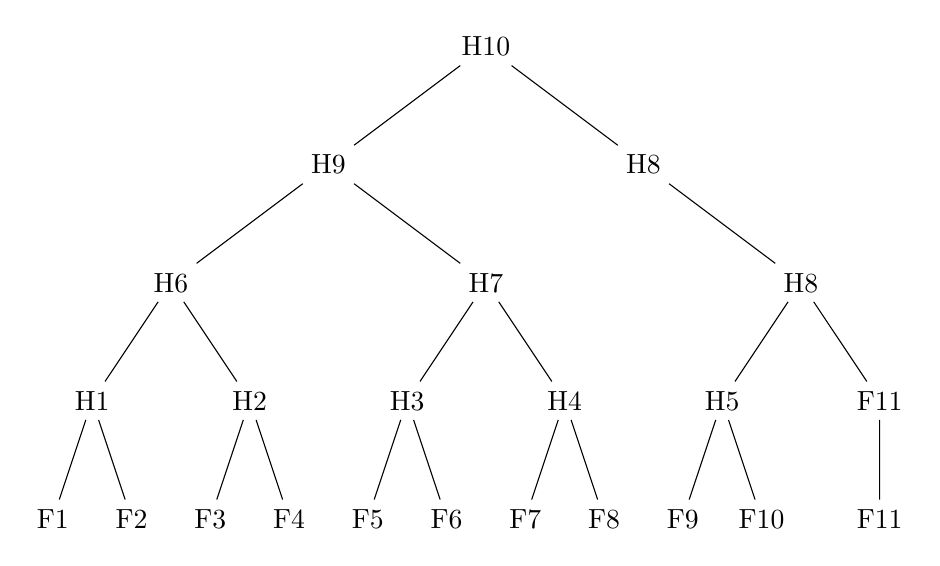
\begin{tikzpicture}[level distance=1.5cm,
        level 1/.style={sibling distance=4cm},
        level 2/.style={sibling distance=4cm},
        level 3/.style={sibling distance=2cm},
        level 4/.style={sibling distance=1cm},
        ]
        \node { H10 }
            child { node { H9 }
                child { node { H6 }
                    child { node { H1 } 
                        child { node { F1 } }
                        child { node { F2 } }
                    }
                    child { node { H2 } 
                        child { node { F3 } }
                        child { node { F4 } }
                    }
                }
                child { node { H7 }
                    child { node { H3 } 
                        child { node { F5 } }
                        child { node { F6 } }
                    }
                    child { node { H4 } 
                        child { node { F7 } }
                        child { node { F8 } }
                    }
                }
            }
            child { node { H8 }
                child [missing]
                child { node { H8 }
                    child { node { H5 } 
                        child { node { F9 } }
                        child { node { F10 } }
                    }
                    child { node { F11 } 
                        child { node { F11 } }
                    }
                }
            };
    \end{tikzpicture}
    \caption{Simple Merkle Tree Example}
    \label{fig:merkle_example}
\end{figure}

In C2PA manifests the initialization segment has one or more trees, each tree consists of thee reference tree layer of the Merkle Tree, a local ID and unique ID, among other data. The two IDs are used to reference the fragments which tree to use. In the fragments themselves there is the list of proofs, a local Id and unique ID, among other data.

\subsection{Validation}

The validation can be either performed only on the initialization segment or on at least one fragment, which requires that initialization segment has also been validated.

The initialization segment contains the C2PA manifest packaged in a \texttt{uuid} BMFF box. In a fragmented BMFF context this manifest contains a \texttt{c2pa.hash.bmff.v2} Assertion. This Assertion contains all relevant information regarding BMFF hashing, like the Merkle Trees, the hash of the initialization segment, hashing algorithm used, the hash exclusion ranges and more. To verify the initialization segment one merely has to read the C2PA manifest and use the included hash exclusion ranges to recreate the hash of the initialization segment. If this hash is equal to the one found in the manifest then the initialization segment is validated as trustworthy.

Each fragment also contains a \texttt{uuid} box. However, the fragments only contain a rudimentary C2PA manifest which holds information required for validation: the proof hashes, the \texttt{local ID} and \texttt{unique ID} and the \texttt{location} on that particular Merkle Tree. The two IDs are required to identify the corresponding Merkle Tree from the C2PA manifest in the initialization segment and the location is the leaf index of the fragment which is needed to determine whether this fragment is the left or child of their parent node.

The validation of a fragment requires the successful validation of the accompanying initialization segment. First step of the validation is calculation of the data hash using the exclusion ranges according to the C2PA manifest. Next the proofs are used in sequence to reconstruct the Merkle Tree. This is done by first determining whether the fragment is a left or right node. The \texttt{location} values begin at zero resulting in an even \texttt{location} representing a left node and an odd \texttt{location} a right node. The first proof is the direct sibling of the fragment. Then the first parent can be calculated using the first proof and the information of \texttt{location} by concatenating the two hashes (left \ right) and hashing the result again using the algorithm specified in the C2PA manifest. This is repeated with the newly created hash and the next proof until all proofs have been used. The final hash resulting from these steps should equal one of the hashes located in the corresponding Merkle Tree from the C2PA manifest. If that is the case the fragment has been validated as trustworthy \footnote{BMFF-Based Hash Validation: \url{https://c2pa.org/specifications/specifications/2.1/specs/C2PA_Specification.html\#_validation}}. A simplified version of the can be seen in pseudo code in \Cref{alg:validate}.

\begin{algorithm}
    \begin{algorithmic}[1]
        \Require $refTreeLayer$ \Comment{remembered from Merkle Tree}
        \State $leafHash \gets hash(leaf)$
        \ForAll{$proof \gets proofs(leave)$}
            \State $leafHash \gets hash(leafHash + proof)$ \Comment{concat order depends on location}
        \EndFor
        \If{leafHash in refTreeLayer}
            \State // leaf is valid
        \Else
            \State // leaf is invalid
        \EndIf
    \end{algorithmic}
    \caption{Validating a Merkle Tree Leaf}
    \label{alg:validate}
\end{algorithm}

\section{Concurrent Approaches}

\todo[inline]{DRM?}
\todo[inline]{Fingerprinting?}
\todo[inline]{Watermarking?}
